\documentclass[preview]{standalone}

\usepackage{amsmath}
\usepackage{amssymb}
\usepackage{bettelini}
\usepackage{stellar}
\usepackage{tikz}
\usepackage{definitions}

\begin{document}

\id{settheory-definitions}
\genpage

\section{Basic definitions}

\begin{snippetdefinition}{set-definition}{Set}
    \todo
\end{snippetdefinition}

\begin{snippetdefinition}{cardinality-definition}{Cardinality}
    The \textit{cardinality} of a \set \(A\), denoted \(|A|\),
    is the amount of elements it contains.
    % Two cardinalities are the same if there is an injective function between them (?)
\end{snippetdefinition}

\begin{snippetdefinition}{subset-definition}{Subset}
    Let \(A\) and \(B\) be \set[sets]. Then, \(A\) is a \textit{subset} of \(B\),
    if all the elements of \(A\) are also in \(B\).
    \[ A \origsubseteq B \]
\end{snippetdefinition}

\begin{snippetdefinition}{proper-subset-definition}{Proper Subset}
    Given two \set[sets] \(A\) and \(B\), if \(A \subseteq B\) but \(A \neq B\),
    then \(A\) is a \textit{proper} (or \textit{strict}) subset of \(B\)
    \[
        A \origsubset B
    \]
\end{snippetdefinition}

\begin{snippetdefinition}{power-set-definition}{Power set}
    Let \(B\) be a \set. Then the \textit{power set} \(\mathcal{P}(B)\)
    is defined as the set of all subsets of \(B\)
    \[
        \mathcal{P}(B)=\{A \suchthat A\subseteq B\}
    \]
\end{snippetdefinition}

\begin{snippetdefinition}{union-definition}{Union}
    If \(A\) and \(B\) are \set[sets], then their \textit{union} is
    \[
        A \cup B = \{x \suchthat x \in A \lor x \in B\}
    \]
\end{snippetdefinition}

\begin{snippetdefinition}{intersection-definition}{Intersection}
    If \(A\) and \(B\) are \set[sets], then their \textit{intersection} is
    \[
        A \cap B = \{x \suchthat x \in A \land x \in B\}
    \]
\end{snippetdefinition}

\begin{snippetdefinition}{difference-definition}{Difference}
    If \(A\) and \(B\) are \set[sets], then their \textit{difference} is
    \[
        A \backslash B = \{x \suchthat x \in A \land x \notin B\}
    \]
\end{snippetdefinition}

\begin{snippet}{set-union-intersection-difference-illustration}
    \begin{center}
        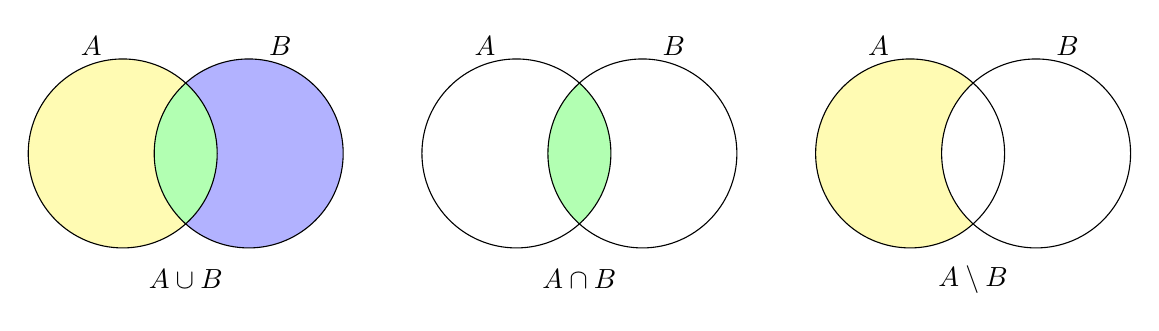
\begin{tikzpicture}
            % Union A ∪ B
            \begin{scope}[shift={(-5,0)}, scale=0.8]
                \fill[yellow!30] (-1,0) circle (1.5);
                \fill[blue!30] (1,0) circle (1.5);
                \begin{scope}
                    \clip (-1,0) circle (1.5);
                    \fill[green!30] (1,0) circle (1.5);
                \end{scope}
                \draw (-1,0) circle (1.5);
                \draw (1,0) circle (1.5);
                \node at (-1.5, 1.7) {$A$};
                \node at (1.5, 1.7) {$B$};
                \node at (0, -2) {$A \cup B$};
            \end{scope}
        
            % Intersection A ∩ B (only middle part)
            \begin{scope}[shift={(0,0)}, scale=0.8]
                \fill[white] (-1,0) circle (1.5);
                \fill[white] (1,0) circle (1.5);
                \begin{scope}
                    \clip (-1,0) circle (1.5);
                    \fill[green!30] (1,0) circle (1.5);
                \end{scope}
                \draw (-1,0) circle (1.5);
                \draw (1,0) circle (1.5);
                \node at (-1.5, 1.7) {$A$};
                \node at (1.5, 1.7) {$B$};
                \node at (0, -2) {$A \cap B$};
            \end{scope}
        
            % Difference A \ B (same as before)
            \begin{scope}[shift={(5,0)}, scale=0.8]
                \fill[yellow!30] (-1,0) circle (1.5);
                \fill[white] (1,0) circle (1.5);
                \begin{scope}
                    \clip (1,0) circle (1.5);
                    \fill[white] (-1,0) circle (1.5);
                \end{scope}
                \draw (-1,0) circle (1.5);
                \draw (1,0) circle (1.5);
                \node at (-1.5, 1.7) {$A$};
                \node at (1.5, 1.7) {$B$};
                \node at (0, -2) {$A \setminus B$};
            \end{scope}
        \end{tikzpicture}
    \end{center}
\end{snippet}

\begin{snippetdefinition}{disjoint-sets-definition}{Disjoint Sets}
    If \(A\) and \(B\) are \set[sets] and \(A \intersection B = \emptyset \), then \(A\)
    and \(B\) are \textit{disjoint sets}.
\end{snippetdefinition}

\begin{snippetdefinition}{cartesian-product-two-sets-definition}{Cartesian Product of two sets}
    [\{
        "generalizations": ["cartesian-product-definition"]
    \}]
    If \(A\) and \(B\) are \set[sets], then their \textit{cartesian product} is
    \[
        A\times B = \{(x,y) \suchthat x \in A \land y \in B\}
    \]
    which is the set of all possible \textit{ordered pairs}.
\end{snippetdefinition}

\begin{snippetdefinition}{cartesian-product-definition}{Cartesian Product}
    Given \(n\) \set[sets] \(A_1, A_2, \ldots, A_2\),
    their \textit{cartesian product} \(A_1 \times A_2 \times \cdots \times A_n\)
    is the set of ordered \(n\)-tuples \((a_1, a_2, \ldots, a_n)\) with \(a_i\in A_i\).
\end{snippetdefinition}

\begin{snippetdefinition}{cartesian-power-definition}{Cartesian Power}
    Let \(n \in \naturalnumbers^\exceptzero\).
    Given a \set \(A\), \(A^n=\underbrace{A \cartesianprod A \cartesianprod \cdots \cartesianprod A}_n\).
\end{snippetdefinition}

\begin{snippet}{n-dimensional-plane-cartesian-power}
    The \(n\)-dimensional plane of real numbers is a cartesian power \({\realnumbers}^n\).
\end{snippet}

%\begin{snippetdefinition}{complement-definition}{Complement}
%    If \(A\) and \(B\) are a \set[sets] where \(A \subseteq B\), its \textit{complement} is
%    \[
%        B \difference A
%    \]
%\end{snippetdefinition}

\begin{snippetdefinition}{disjoint-union-definition}{Disjoint union}
    Given \set[sets] \(A_{i\in I}\), their disjoint union is
    \[
        \bigsqcup_{i\in I}A_i= \bigcup_{i\in I}\{(x, i) \suchthat x \in A_i\}
    \]
    which consists of prdered pairs where the second element
    is the index of the set.
\end{snippetdefinition}

\end{document}
